\chapter{Progettazione e sviluppo del modulo \texttt{nfproxy}}\label{chap:nfproxy}

Il \gls{regex} filtering è un modello di filtraggio che garantisce ottime prestazioni (grazie all'elaborazione tramite linguaggi e librerie ottimizzati), ma presenta forti limitazioni nella flessibilità di analisi del traffico.
Questa rigidità è particolarmente rilevante nei \gls{ctf}, dove la maggior parte dei servizi utilizza protocolli come \gls{http}, che spesso includono contenuti compressi o codificati (e.g., Base64, gzip), difficilmente analizzabili tramite \gls{regex}.
A discapito delle prestazioni, \texttt{\gls{nfproxy}} introduce il vantaggio di scrivere filtri in Python\footcite{\url{https://python.org/}}{python}, linguaggio semplice e rapido per lo scripting offrendo:

\begin{itemize}
    \setlength{\itemsep}{4pt}
    \setlength{\parskip}{4pt}
    \item Massima libertà nell'implementazione delle logiche di filtraggio;
    \item Prestazioni che, nonostante l'utilizzo di codice interpretato, restano elevate anche grazie a scelte architetturali mirate;
    \item Supporto nativo agli algoritmi di compressione e codifica più comuni, mediante il \textit{parsing} del protocollo applicativo.
\end{itemize}

\texttt{\gls{nfproxy}} non è un proxy tradizionale ma un modulo basato su
\gls{nfqueue}\footcite{\url{https://netfilter.org/projects/libnetfilter_queue/}}{netfilter_queue},
che permette un controllo sul traffico paragonabile ad un proxy classico, ma con accesso diretto ai pacchetti a livello di rete (layer 3/4) e con un'intercettazione del traffico invisibile all'applicativo.
Va riportata l'esistenza di limitazioni nella modifica dei pacchetti, che tuttavia non rappresenta un caso d'uso tipico della difesa del servizio.

Il sistema combina C++ per una gestione efficiente dei pacchetti e Python per eseguire il \textit{parsing} dei protocolli applicativi.
Questo approccio ibrido permette di sfruttare al meglio le caratteristiche di entrambi i linguaggi, garantendo prestazioni elevate e flessibilità nello sviluppo dei filtri.

I protocolli attualmente supportati includono:
\begin{itemize}
    \setlength{\itemsep}{4pt}
    \setlength{\parskip}{4pt}
    \item \gls{http}/1.1\footcite{RFC2616, Hypertext Transfer Protocol -- HTTP/1.1}{rfc2616} (con gestione compressione/encoding del body);
    \item Websocket\footcite{RFC6455, The WebSocket Protocol}{rfc6455} (con decodifica dei frame e supporto alle estensioni);
    \item \gls{tcp} standard\footcite{RFC9293, Transmission Control Protocol (TCP)}{rfc9293} (con ricostruzione dello stream).
\end{itemize}

\section{Scelte progettuali}

Di seguito gli obiettivi fondamentali del modulo:

\begin{itemize}
    \setlength{\itemsep}{4pt}
    \setlength{\parskip}{4pt}

    \item \textbf{Integrazione con Python}: Fornire un'interfaccia in Python per implementare le regole di filtraggio, con funzioni ottimizzate e sintassi intuitiva;

    \item \textbf{Analisi avanzata di \gls{http}/1.1 e WebSocket}: Interpretazione nativa dei pacchetti applicativi, con estrazione automatica dei dati decodificati/decompressi. Supporto integrato per:
    gzip\footcite{RFC1952, GZIP file format specification version 4.3}{rfc1952},
    deflate\footcite{RFC1951, DEFLATE Compressed Data Format Specification version 1.3}{rfc1951},
    brotli\footcite{RFC7932, Brotli Compressed Data Format}{rfc7932},
    zstd\footcite{RFC8478, Zstandard Compression and the application/zstd Media Type}{rfc8478},
    e l'estensione WebSocket permessage-deflate\footcite{RFC7692, Compression Extensions for WebSocket}{rfc7692};

    \item \textbf{Ricostruzione dello stream TCP}: Accesso al payload ordinato a livello di trasporto, indipendentemente dalla frammentazione;

    \item \textbf{Manipolazione degli header}: Lettura e modifica diretta dei campi negli header di rete (\gls{ip}) e trasporto (\gls{tcp});

    \item \textbf{Compatibilità dual-stack}: Elaborazione sia di pacchetti \gls{ipv4}\footcite{RFC791, Internet Protocol}{rfc791} che \gls{ipv6}\footcite{RFC2460, Internet Protocol, Version 6 (\gls{ipv6}) Specification}{rfc2460};

    \item \textbf{Allocazione e deallocazione di memoria ottimizzata}: Gestione automatica dei buffer per evitare memory leak e sovraccarichi, non delegandone la gestione al programmatore, ma fornendo opzioni di configurazione opzionali per configurare il modo in cui vengono gestiti;

    \item \textbf{Diagnostica avanzata}: Notifica strutturata degli errori (codici, descrizioni, contesto) con log dettagliati per l'analisi forniti in tempo reale;

    \item \textbf{Modifica dinamica delle regole}: Attivazione/disattivazione istantanea dei filtri (anche solo di alcuni specifici) senza interrompere il servizio;

    \item \textbf{Elaborazione parallela}: Distribuzione del carico su multipli core della \gls{cpu} per garantire scalabilità lineare;

    \item \textbf{Validazione dei filtri tramite simulazione}: Verifica delle regole in un ambiente simulato per debugging da poter utilizzare in fase di sviluppo e verifica dei filtri.
\end{itemize}

\vspace{\fill}
\newpage

\section{Architettura}

Il modulo \texttt{\gls{nfproxy}} viene avviato dal backend di Firegex attraverso un processo articolato in tre fasi principali.

In primo luogo, il backend configura le regole di \gls{nftables}\footcite{\url{https://netfilter.org/projects/nftables/}}{nftables} mediante chiamate alle sue \gls{api} \gls{json}.\@ Successivamente, viene inizializzato il componente C++ responsabile della logica centrale, che include la gestione del multi-threading, l'elaborazione a basso livello dei pacchetti e la ricostruzione degli stream \gls{tcp}.\@ Nella fase finale, vengono caricati e applicati dinamicamente i filtri Python definiti dall'utente. L'architettura completa del modulo è rappresentata nella Figura~\ref{fig:firegex_nfproxy_arch}, dove si evince l'interazione tra i tre livelli (configurazione, core C++ e strato Python).

\begin{figure}[H]
    \centering
    \includesvg[width=0.90\textwidth]{images/chapter3/nfproxy.drawio.svg}
    \caption{Architettura del modulo \gls{nfqueue}.}\label{fig:firegex_nfproxy_arch}
\end{figure}

\section{Elaborazione parallelizzata dei pacchetti}

Uno dei principali ostacoli progettuali ha riguardato la parallelizzazione dei processi di elaborazione, legata a tre fattori critici:
il funzionamento intrinseco di \gls{nfqueue}, alcune peculiarità del linguaggio Python e l'integrazione ibrida C++/Python.

Tre obiettivi hanno guidato l'implementazione della parallelizzazione:

\begin{itemize}
    \setlength{\itemsep}{2pt}
    \setlength{\parskip}{2pt}
    \item \textbf{Isolamento dei dati tra processi}: Prevenire conflitti interprocesso per evitare corruzione dati, crash imprevisti e comportamenti anomali;
    \item \textbf{Minimizzazione dei lock}: Limitare l'uso di meccanismi di blocco (pur necessari per risorse condivise) per prevenire deadlock e un degrado delle prestazioni;
    \item \textbf{Ottimizzazione della memoria}: Eliminare copie ridondanti dei pacchetti e processi superflui, massimizzando throughput e riducendo la latenza.
\end{itemize}

La soluzione adottata segue il pattern \textit{producer-consumer}. Un processo produttore unico, responsabile del binding alla \gls{nfqueue},
riceve i pacchetti dal kernel e li distribuisce a multiple code \gls{fifo}.\@ I consumatori, associati ciascuno ad una coda dedicata, gestiscono in parallelo:
\begin{itemize}
    \setlength{\itemsep}{2pt}
    \setlength{\parskip}{2pt}
    \item Ordinamento dei pacchetti \gls{tcp};
    \item Applicazione dei filtri Python;
    \item Invio dei verdicts\footcite{\url{https://netfilter.org/projects/libnetfilter_queue/doxygen/html/group__nfq__verd.html}}{vedicts_nfqueue} al kernel.
\end{itemize}

L'unica sezione critica risiede nell'accesso concorrente alle code, protetto da un sistema di lock basato su
std::mutex\footcite{\url{https://en.cppreference.com/w/cpp/thread/mutex}}{std_mutex} e std::condition\_variable\footcite{\url{https://en.cppreference.com/w/cpp/thread/condition_variable}}{condition_variable_std}. Questa scelta, preferita alle unix pipe\footcite{\url{https://man7.org/linux/man-pages/man2/pipe.2.html}}{unix_pipe} per motivi prestazionali, implementa inoltre un meccanismo di backpressure che blocca il produttore in caso di code sature, prevenendo un consumo eccessivo di memoria.

L'implementazione si basa su quella pubblicata da Arif Jaffer\footcite{\url{https://www.bit-byter.com/blog/files/blocking-q-cpp.html}}{blocking_queue_cpp} per le code bloccanti.

\subsection{A Per-Interpreter Global Interpreter Lock}

Una problematica riguardo la parallelizzazione riguarda una caratteristica del linguaggio Python: il \gls{gil}\footcite{\textit{Understanding the python gil}}{beazley2010understanding}. Questo meccanismo limita l'utilizzo dei thread consentendo l'esecuzione di un solo thread alla volta, necessario per prevenire conflitti nella gestione interna degli oggetti Python (come per il \textit{reference counting}) che non è implementata in modo \textit{thread-safe}.

Si osserva inoltre come, in questo specifico contesto, Python gestisca operazioni \textit{\gls{cpu}-bound}, accentuando ulteriormente gli svantaggi del \gls{gil}.
In Figura~\ref{fig:py_gil_schema} è possibile visualizzare uno schema estratto da \textit{Understanding the python gil}\footciteref{beazley2010understanding} che descrive il funzionamento del Python \gls{gil}

\begin{figure}[H]
    \centering
    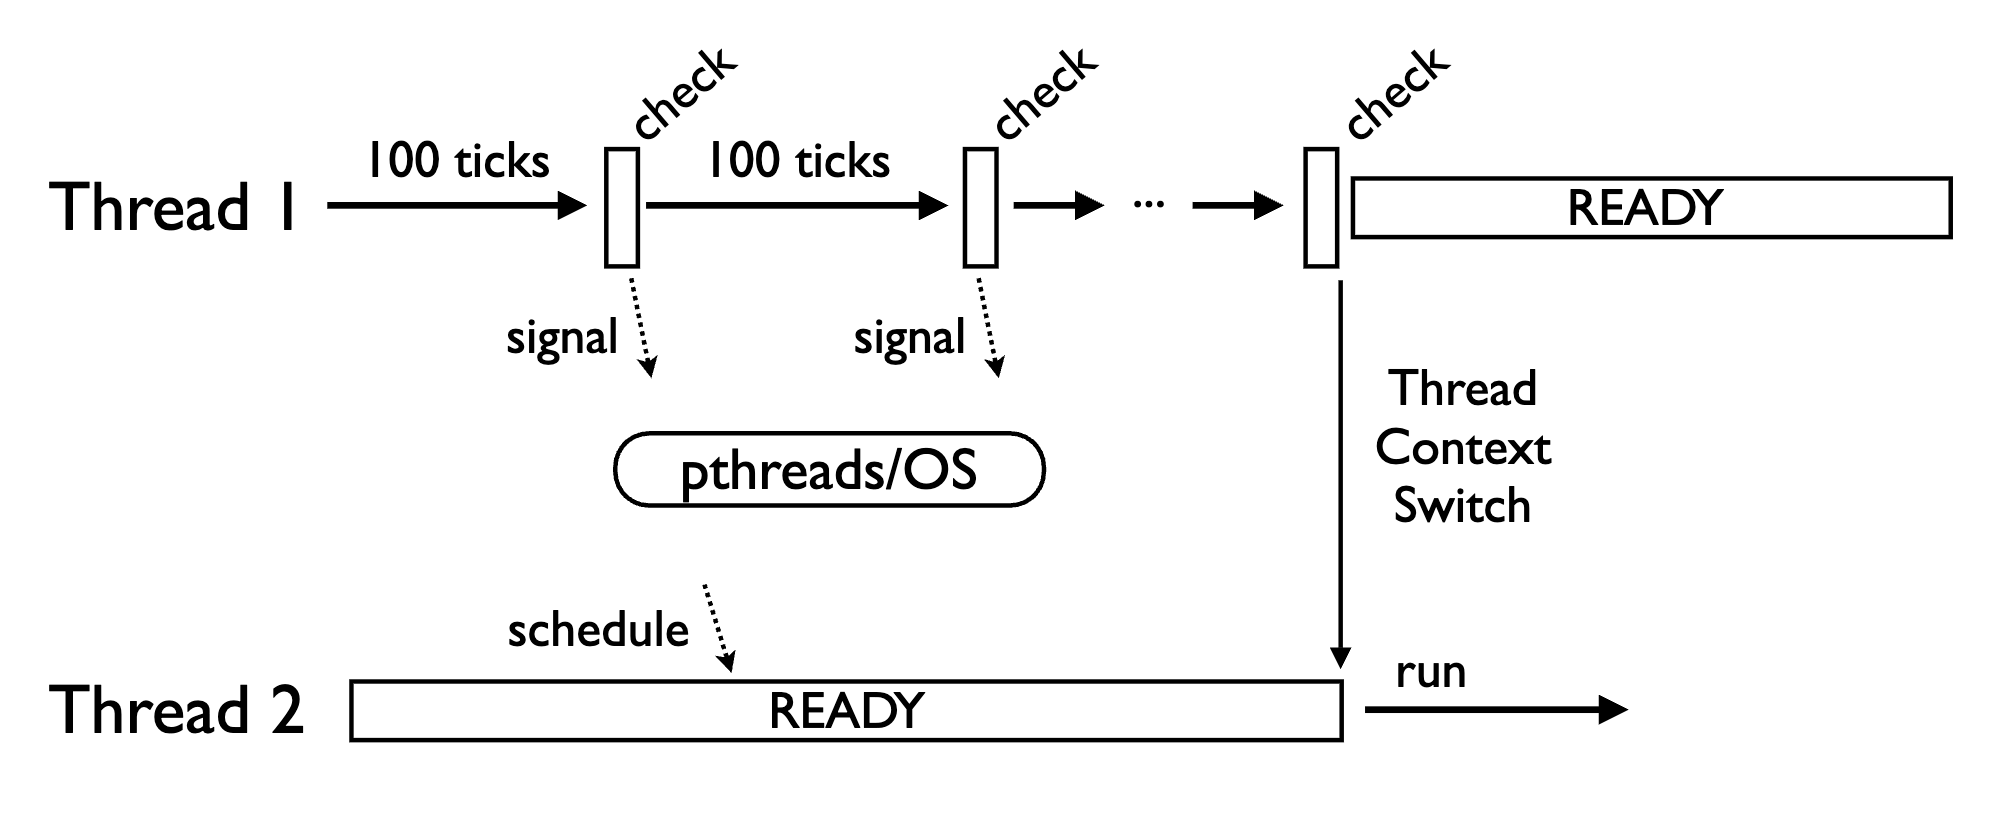
\includegraphics[width=0.98\textwidth]{images/chapter3/GIL.png}
    \caption{Python Global Interpreter Lock\footciteref{beazley2010understanding}.}\label{fig:py_gil_schema}
\end{figure}

Una soluzione alternativa potrebbe essere l'uso di processi multipli (con \gls{gil} separati per processo), approccio che tuttavia introdurrebbe overhead dovuti
alla comunicazione inter-processo e alla duplicazione della memoria.

La soluzione adottata sfrutta il \gls{pep} 684\footcite{\url{https://peps.python.org/pep-0684/}}{pep648} introdotto in Python 3.12, che permette l'esecuzione
di interpreti Python indipendenti nello stesso processo, ciascuno con il proprio \gls{gil}.\@ L'attivazione di questa funzionalità avviene esclusivamente tramite C-\gls{api}, consentendo:
\begin{itemize}
    \setlength{\itemsep}{2pt}
    \setlength{\parskip}{2pt}
    \item Avvio diretto di interpreti via libpython;
    \item Integrazione trasparente tra codice C++ e Python;
    \item Parallelismo reale senza overhead di processi multipli.
\end{itemize}
L'impossibilità di condividere oggetti tra interpreti, uno dei limiti di questo approccio, non costituisce un problema nel nostro caso poiché, grazie al meccanismo di
smistamento dei pacchetti descritto nel prossimo paragrafo, ciò non sarà necessario.

L'eseguibile C++ una volta avviato, sarà in attesa del codice python da utilizzare come filtro: una volta arrivato il codice, questo viene compilato in bytecode tramite la funzione \texttt{compile} integrata in python e successivamente, al fine di rendere duplicabile il bytecode compilato nei vari interpreti inizializzati, ne eseguiamo il marshaling\footcite{\url{https://docs.python.org/3/library/marshal.html}}{marshal_python}, ottenendone una rappresentazione seria.
Come mostrato nel Codice~\ref{lst:no_gil_python_nfproxy}, i thread designati all'analisi e al filtraggio delle connessioni, nella loro inizializzazione eseguiranno le procedure indicate nella documentazione delle C \gls{api} di Python per creare un \gls{gil} indipendente da quello principale, e poi deserializzeranno il bytecode del filtro in python.
Per nuovi aggiornamenti del filtro i thread si occuperanno deserializzare il nuovo bytecode una volta disponibile.
\begin{listing}[H]
\begin{minted}[
    frame=single,
    framerule=0.8pt,
    fontsize=\footnotesize,
    breaklines
]{cpp}
// Configurazione interprete con GIL indipendente
PyInterpreterConfig py_thread_config = {
    .use_main_obmalloc = 0,
    .allow_fork = 0,
    .allow_exec = 0,
    .allow_threads = 0,
    .allow_daemon_threads = 0,
    .check_multi_interp_extensions = 1,
    .gil = PyInterpreterConfig_OWN_GIL,
};

void before_loop() {
    PyStatus pystatus;
    tstate = PyThreadState_New(PyInterpreterState_Main());
    PyEval_AcquireThread(tstate); // Acquisizione GIL
    // Creazione del GIL indipendente + rilascio di quello principale
    pystatus = Py_NewInterpreterFromConfig(&tstate, &py_thread_config);
    handle_packet_code = unmarshal_code(...); // Deserializzazione bytecode
}
\end{minted}
\vspace{-1em}
\caption{Inizializzazione di un processo consumatore con GIL indipendente in \texttt{nfproxy}.}\label{lst:no_gil_python_nfproxy}
\end{listing}

Per ogni nuova connessione \gls{tcp} inoltre, vengono eseguite le seguenti operazioni:
\begin{itemize}
    \setlength{\itemsep}{2pt}
    \setlength{\parskip}{2pt}
    \item Viene inizializzato un nuovo contesto globale Python dedicato a questa connessione;
    \item Viene eseguito il bytecode su questo contesto per inizializzare i filtri;
    \item Continuiamo a usare contesto inizializzato per eseguire le procedure di analisi e filtraggio del traffico (nel contesto sono inclusi i buffer necessari al \textit{parsing});
    \item Al termine della connesione, deallochiamo il contesto globale creato.
\end{itemize}

L'utilizzo delle funzionalità offerte dal \gls{pep} 684\footcite{\url{https://peps.python.org/pep-0684/}}{pep648}, soffre tuttavia anche di forti limitazioni sull'utilizzo di moduli senza multi-phase initialization\footcite{\url{https://peps.python.org/pep-0489/}}{pep489} (includendo tutti quelli scritti in Cython\footcite{\url{https://cython.org/}}{cython}) e moduli con componenti non \textit{thread-safe}. Nel corso dello sviluppo, queste limitazioni sono state oggetto di diverse problematiche, affrontate e approfondite in seguito.

Un'altra possibilità considerata è stata l'utilizzo dell'interprete in \textit{free-threaded} mode di Python 3.13\footcite{\url{https://docs.python.org/3/whatsnew/3.13.html\#whatsnew313-free-threaded-cpython}}{py13_free_threaded}, attualmente sconsigliato per:
\begin{itemize}
    \setlength{\itemsep}{2pt}
    \setlength{\parskip}{2pt}
    \item Lo stato sperimentale della feature;
    \item Calo prestazionale dovuto alla disattivazione temporanea di alcuni sistemi di ottimizzazione del linguaggio;
    \item Incompatibilità con molti moduli CPython.
\end{itemize}

\subsection{Bilanciamento del carico}\label{custom_balancing_system}

Per il bilanciamento del carico tra i processi consumatori, finalizzato all'isolamento e alla distribuzione equa dei pacchetti, è stato implementato un meccanismo di hashing basato su indirizzi \gls{ip} e porte di origine/destinazione mostrato nel Codice~\ref{lst:nfproxy_hash}. Questo approccio garantisce una distribuzione uniforme dei pacchetti tra i consumatori, evitando sovraccarichi e assicurando un'elaborazione parallela efficiente, oltre che a instradare i pacchetti di una stessa connessione sempre verso lo stesso thread. Il seguente meccanismo è stato re-integrato anche nel modulo \texttt{nfproxy} e anche progettato anche per essere facilmente utilizzato in futuri moduli di Firegex.

\begin{listing}[H]
\begin{minted}[
    frame=single,
    framerule=0.8pt,
    fontsize=\footnotesize,
    breaklines
]{cpp}
uint32_t hash_stream_id(const stream_id &sid) {
    uint32_t addr_hash = 0;
    addr_hash ^= min_addr[0] ^ min_addr[1] ^ min_addr[2] ^ min_addr[3];
    addr_hash ^= max_addr[0] ^ max_addr[1] ^ max_addr[2] ^ max_addr[3];
    uint32_t ports = (static_cast<uint32_t>(sid.min_address_port) << 16) | sid.max_address_port;
    uint32_t hash = addr_hash ^ ports;
    hash *= 0x9e3779b9; // Entropia nell'hashing
    return hash;
}
void balancer(PktRequest<Worker>* pkt) {
    const size_t idx = hash_stream_id(pkt->sid) % pkt->ctx->size();
    converted_pkt->ctx->queue.put(converted_pkt);
}
\end{minted}
\vspace{-1em}
\caption{Funzione di hashing per stream\_id (valida per IPv4/IPv6) in \texttt{\gls{nfproxy}}.}\label{lst:nfproxy_hash}
\end{listing}

La tecnica riprende i meccanismi di bilanciamento usati kernel space da \gls{nfqueue}, che tuttavia non considera le porte di origine/destinazione,
limitandosi ad un hashing basato solo sugli indirizzi \gls{ip} come mostrato nel Codice~\ref{lst:nfqueue_hash_linux}.\@ Ciò è dovuto alla necessità di adattare l'algoritmo anche a protocolli diversi da \gls{tcp} e \gls{udp}, come \gls{icmp} che non prevede porte.

\begin{listing}[H]
\begin{minted}[
    frame=single,
    framerule=0.8pt,
    fontsize=\footnotesize,
    breaklines
]{cpp}
u32 nfqueue_hash(sk_buff *skb, u16 queue, u16 queues_total, u8 family,
    u32 initval) {
    switch (family) {
    case NFPROTO_IPV4:
        queue += reciprocal_scale(hash_v4(ip_hdr(skb), initval), queues_total);
        break;
    case NFPROTO_IPV6:
        queue += reciprocal_scale(hash_v6(ipv6_hdr(skb), initval), queues_total);
        break;
    }
    return queue;
}
\end{minted}
\vspace{-1em}
\caption{funzione nfqueue\_hash dal kernel Linux (semplificata) (versione 6.14-rc7).}\label{lst:nfqueue_hash_linux}
\end{listing}

L'esclusione delle porte nell'hashing kernel\footcite{\texttt{nfqueue\_hash}, hash function for \texttt{nf\_queue} in the Linux kernel}{nfqueue_ip_hashing}
nel sistema di \textit{balancing}\footcite{\texttt{nfqueue\_tg\_v3}, balancing function for \texttt{nf\_queue} in the Linux kernel}{nfqueue_ip_balancing} integrato in \gls{nfqueue}
rappresenta un limite critico in scenari \gls{ctf} con \gls{nat}, dove tutto il traffico anonimizzato verrebbe gestito da un singolo consumatore.
Questo è il motivo che ha spinto alla scelta di un approccio più sofisticato, che garantisce un effettivo bilanciamento del carico sui vari thread.

Alcuni benchmark eseguiti sul sistema di bilanciamento sono disponibili nel Capitolo~\ref{balancing_benchmark}

\section{Parsing dei pacchetti L3}

All'arrivo dei pacchetti nella \gls{nfqueue}, viene eseguita un'analisi immediata del protocollo di livello 3 mediante ispezione dei primi
4 bit del campo version, valida sia per IPv4 che \gls{ipv6}. Identificata la versione \gls{ip}, il \textit{parsing} multilivello viene delegato a
libtins\footcite{\url{https://libtins.github.io/}}{libtins}, che ricostruisce ricorsivamente gli header di rete e trasporto.

Anche questa parte come per il bilanciamento del carico, è progettata per essere facilmente utilizzata in futuri moduli di Firegex, e re-integrata anche per il modulo \texttt{nfregex} (che supporta anche i pacchetti UDP, che pertanto vengono considerati in questo paragrafo).

La libreria genera automaticamente lo stream\_id, struttura dati univoca per identificare connessioni TCP/UDP attraverso
una coppia di tuple (\gls{ip}:porta) sorgente/destinazione, che sono ordinate considerando la singola tupla come unica entità, e quindi non slegando mai
\gls{ip} e porta tra loro. Questo approccio permette di identificare univocamente una connessione, indipendentemente dalla direzione del traffico (ingresso/uscita). La fase di analisi del pacchetto tramite libtins\footcite{\url{https://libtins.github.io/}}{libtins} è eseguita dal costruttore della classe \texttt{PktRequest} mostrata nel Codice~\ref{lst:pktrequest_constructor}.

\begin{listing}[H]
\begin{minted}[
    frame=single,
    framerule=0.8pt,
    fontsize=\footnotesize,
    breaklines
]{cpp}
PktRequest(const char* payload, size_t plen, T* ctx, mnl_socket* nl,
           nfgenmsg *nfg, nfqnl_msg_packet_hdr *ph, bool is_input):
    ctx(ctx), nl(nl), res_id(nfg->res_id),
    packet_id(ph->packet_id), is_input(is_input),
    packet(string(payload, plen)),
    action(FilterAction::NOACTION),
    is_ipv6((payload[0] & 0xf0) == 0x60) // Verifica versione IP
{
    if (is_ipv6){
        ipv6 = new Tins::IPv6((uint8_t*)packet.c_str(), plen); // Parsing IPv6
        sid = stream_id::make_identifier(*ipv6); // Generazione stream_id
        _original_size = ipv6->size();
    }else{
        ipv4 = new Tins::IP((uint8_t*)packet.c_str(), plen); // Parsing IPv4
        sid = stream_id::make_identifier(*ipv4);
        _original_size = ipv4->size();
    }
    l4_proto = fill_l4_info(); // Estrazione info layer 4
}
\end{minted}
\vspace{-1em}
\caption{Costruttore di PktRequest e \textit{parsing} nel pacchetto di rete in firegex.}\label{lst:pktrequest_constructor}
\end{listing}

Inoltre, lo stream\_id è indipendente dal protocollo internet utilizzato, identificando anche connessioni miste IPv4/IPv6 (usando indirizzi IPv6 \textit{IPv4-Compatible}): questo permette di utilizzare la stessa queue per interfaccie di rete differenti, caratteristica potenzialmente utile per implementare nuove feature sulla selezione del traffico da inoltrare alla queue.

Ogni produttore utilizza questo dato come chiave per individuare i dati relativi ad una specifica connessione, salvandoli in una std::map\footcite{\url{https://en.cppreference.com/w/cpp/container/map}}{std_map} diversa per ogni singolo produttore, così implementabile per merito del meccanismo di smistamento dei pacchetti descritto nel Capitolo~\ref{custom_balancing_system}.
Il produttore, ricevuto il pacchetto, lo ingloba in un oggetto PktRequest, che contiene tutte le informazioni necessarie per l'elaborazione del pacchetto, e lo inserisce nella coda condivisa del produttore di riferimento.
Sarà il produttore che una volta elaborato il pacchetto ed inviato il verdetto al kernel, deallocherà questa struttura passando all'elaborazione del prossimo pacchetto. Nessuna copia in memoria è pertanto necessaria in questo passaggio.

\section{Gestione dei pacchetti TCP}

Prima di inizializzare la queue, vengono (dal backend python) inserite tramite \gls{nftables} le regole per intercettare il traffico in un certo punto della catena di netfilter, per essere mandato alla queue che determinerà un verdetto sul pacchetto.

Il traffico in particolare viene intercettato sia in \texttt{pre-routing}, che in \texttt{post-routing} ad un hook prima dell'azione del modulo \texttt{conntrack}, ma dopo dell'azione di defrag, rispettivamente a \texttt{prio} -310 in \texttt{pre-routing} e 110 in \texttt{post-routing} rientrando nei range corretti, come riportati sulla wiki ufficiale di \gls{nftables}\footcite{\url{https://wiki.nftables.org/wiki-nftables/index.php/Netfilter_hooks}}{netfilter_hooks}. Questo permette di ottenere dei pacchetti che hanno già subito il processo di deframmentazione a livello 3, di cui pertanto non ci dovremo preoccupare, ma che non hanno subito il processo di routing (che quindi volendo potremmo manipolare) e che non sono stati ancora analizzati dal modulo \texttt{conntrack}.
Tuttavia, qui i pacchetti non hanno subito il processo di ordinamento dei payload che avviene a livello 4, sul quale come è possibile osservare dalla Figura~\ref{fig:nftables_hooks}, non è possibile intercettare del traffico, poiché i pacchetti arriveranno direttamente alle fasi di gestioni dei dati per la loro consegna alla socket a livello applicatvo.
Pertanto è dato a noi il compito di analizzare il traffico, ordinando i pacchetti \gls{tcp} per un'utilizzo dei dati coerente a quelli che saranno letti dall'applicazione.
Libtins semplifica significativamente questa gestione attraverso meccanismi automatizzati gestiti dal suo \gls{tcp} follower\footcite{Esempio \gls{tcp} Follower: \url{https://libtins.github.io/examples/http-requests/}}{libtins_tcp_follower_gh} per:
\begin{itemize}
    \setlength{\itemsep}{2pt}
    \item Chiusura dei flussi \gls{tcp} basata su:
    \begin{itemize}
        \setlength{\itemsep}{1pt}
        \item Analisi del traffico (flag FIN/RST);
        \item Timeout configurabili (rilevamento di inattività);
        \item Utilizzo eccessivo dei buffer di memoria.
    \end{itemize}
    \item Ricostruzione dello stream da segmenti non ordinati (o duplicati);
    \item Gestione automatica della memoria utile alla ricostruzione.
\end{itemize}
Il follower inoltre permette facilmente l'integrazione di dati gestiti esternamente, tramite il suo sistema di callback, che ne chiamerà le funzionalità compatibilmente con quanto fatto con i buffer internamente.
Le callback permettono di gestire le seguenti operazioni:
\begin{itemize}
    \setlength{\itemsep}{2pt}
    \item Inizializzazione contesti;
    \item Pulizia risorse;
    \item Propagazione di eventi critici (per chiusure anomale dei flussi).
\end{itemize}

Ogni processo consumatore ha un suo follower dedicato che analizzerà i flussi relativi alla porzione traffico a lui dedicata.

\section{Modifica dei pacchetti}

Il modulo \gls{nfqueue} consente effettivamente la modifica dei pacchetti, mediante l'invio al kernel Linux del pacchetto modificato, offrendo la possibilità di alterare header
\gls{ip}, \gls{tcp} ed il relativo payload. Tuttavia la funzionalità di modifica in \texttt{nfproxy} è stata implementata solo parzialmente e non risulta pienamente affidabile.

Le limitazioni derivano da problematiche intrinseche legate all’interazione con i meccanismi di livello di trasporto. Ad esempio, modifiche al payload \gls{tcp} durante connessioni attive potrebbero invalidare checksum o causare inconsistenze nei \gls{seq}. La complessità per garantire coerenza in tutti i possibili scenari (come in caso di ritrasmissioni) rende l’implementazione robusta di questa feature particolarmente onerosa. Inoltre, se gestita male, la modifica del payload potrebbe essere soggetta a vulnerabilità di sicurezza. Valutando il rapporto rischio-beneficio, si è optato per comunque rendere disponibile la funzionalità, seppur parzialmente implementata, ma fortemente disincentivata e volutamente resa meno facilmente accessibile.

L’effettiva necessità operativa risulta infatti marginale nella maggior parte degli scenari \gls{ctf}, mentre i potenziali effetti collaterali verrebbero a compromettere uno degli obiettivi principali: la stabilità del servizio.

Di seguito si riporta una descrizione accurata delle problematiche riscontrate e delle soluzioni proposte, o applicate con relativi limiti e valutazioni rischio/beneficio.
Le problematiche sul calcolo dei campi di integrità dei dati non sono trattate, ma considerate già risolte tramite l'utilizzo di libtins, che si occupa durante la serializzazione del pacchetto di ricalcolare questi campi nei vari layer interessati, pertanto non considerata una problematica rilevante.

L'unica operazione aggiuntiva affrontata su questo, è stata la necessità di reinserire il payload del pacchetto nella catena di \gls{pdu} di libtins, poiché (seppur non documentato), il follower del flusso \gls{tcp} internamente separa di fatto il payload dal pacchetto\footcite{Libtins, istruzione per la separazione del payload nel follower (std::move del payload)}{libtins_payload_move_gh}, rendendone necessario il reinserimento per la corretta serializzazione e calcolo di questi campi.

\subsection{Cambio di dimensione del payload}

Come emerge dalle specifiche stesse del protocollo di trasporto \gls{tcp}\footcite{RFC9293, Transmission Control Protocol (TCP)}{rfc9293}, questo tiene traccia dello stato della corretta recezione dei pacchetti tramite un meccanismo di piggybacking che fa utilizzo dei campi numerici \gls{ack} e \gls{seq}.
Nella trasmissione, il \gls{seq} indica il byte da cui inizia il payload del pacchetto relativamente alla sua posizione nello stream, mentre il campo \gls{ack} della risposta di conferma proveniente dal ricevente, indica fino a che punto il flusso di dati è stato ricevuto correttamente.

Questo meccanismo è fondamentale per il corretto funzionamento del protocollo e per la corretta ricostruzione del flusso originale: di conseguenza la modifica alla dimensione del payload causa inevitabilmente l'incoerenza di questi valori che porteranno a comportamenti inaspettati, non conformi al normale funzionamento del protocollo.

Per risolvere la problematica descritta, è stato implementato un sistema di traduzione bidirezionale dei campi \gls{seq} e \gls{ack}.

Questo meccanismo tenta di mantenere la coerenza logica della comunicazione riconvertendo i valori modificati in modo da preservare la corrispondenza tra la dimensione originale dei pacchetti e le aspettative del client (e viceversa del server).
Il kernel e il \gls{tcp} Follower di libtins ricevono così numerazioni coerenti con le alterazioni applicate, mantenendo la sincronizzazione degli stati di connessione.
Il sistema opera in modo simmetrico per entrambe le direzioni del traffico: le modifiche applicate ai pacchetti in uscita vengono compensate da una riconversione inversa per quelli in entrata. L'attivazione avviene automaticamente alla prima modifica di un pacchetto nella sessione \gls{tcp} e rimane attiva per tutta la durata della connessione, garantendo la persistenza del contesto di traduzione.

Questa conversione avviene tramite il calcolo incrementale dell'offset che intercorre tra la dimensione del flusso originale e la dimensione del flusso modificato come mostrato nel Codice~\ref{lst:tcp_ack_seq_transl}.

\begin{listing}[H]
\begin{minted}[
    frame=single,
    framerule=0.8pt,
    fontsize=\footnotesize,
    breaklines
]{cpp}
size_t payload_offset = data_size() - _data_original_size;
if (is_input){ // Inbound packet
    ack_seq_offset->in += payload_offset;
}else{
    ack_seq_offset->out += payload_offset;
}
\end{minted}
\vspace{-1em}
\caption{Calcolo dell'offset cumulativo nello stream TCP da correggere in modifica.}\label{lst:tcp_ack_seq_transl}
\end{listing}
A seguito della modifica, nei prossimi pacchetti vengono compatibilmente ricalcolati gli \gls{ack} e \gls{seq}, su tutto il traffico come mostrato nel Codice~\ref{lst:tcp_ack_seq_transl_fixing}.
\begin{listing}[H]
\begin{minted}[
    frame=single,
    framerule=0.8pt,
    fontsize=\footnotesize,
    breaklines
]{cpp}
if (is_input){ // Inbound packet
    tcp->seq(tcp->seq() + ack_seq_offset->in);
    tcp->ack_seq(tcp->ack_seq() - ack_seq_offset->out);
}else{
    tcp->ack_seq(tcp->ack_seq() - ack_seq_offset->in);
    tcp->seq(tcp->seq() + ack_seq_offset->out);
}
\end{minted}
\vspace{-1em}
\caption{Algoritmo di traduzione di ACK e SEQ numbers a seguito di mangle dei pacchetti.}\label{lst:tcp_ack_seq_transl_fixing}
\end{listing}
Un'analisi preliminare e dei test preliminari, suggerirebbero l'adeguatezza di questa soluzione. Tuttavia, a seguito di analisi più accurate, si evince come il meccanismo presenti limitazioni intrinseche in determinate casistiche di traffico. L'approccio risulta efficace esclusivamente in condizioni ideali di trasmissione, dove non si verificano fenomeni di ritrasmissione di pacchetti.

La criticità principale risiede nell'algoritmo di conversione, che non considera adeguatamente le ritrasmissioni di segmenti antecedenti al pacchetto modificato. In tali scenari, il ricalcolo dell'\gls{ack} relativo richiederebbe l'utilizzo di un offset compatibile non all'ultimo offset calcolato, ma allo stato del flusso nella parte interessata dalla ritrasmissione, operazione che l'implementazione corrente non esegue. La problematica è diretta conseguenza della mancanza di un analisi del traffico contestuale, capace di identificare la porzione di flusso effettivamente coinvolta nella ritrasmissione, e di memorizzare le discrepanze cumulative associandole direttamente alle varie parti dello stream interessate.
\begin{figure}[H]
    \centering
    \includesvg[width=0.90\textwidth]{images/chapter3/TCP_ack_seq_transl_failure.drawio.svg}
    \caption{Esempio di una possibile problematica nella traduzione di \gls{ack} e \gls{seq} implementata.}\label{fig:tcp_ack_seq_transl_failure}
\end{figure}
L'analisi della Figura~\ref{fig:tcp_ack_seq_transl_failure} evidenzia come le casistiche descritte possano compromettere integralmente il sistema di traduzione implementato. Tali scenari, particolarmente probabili in condizioni di congestione di rete, rappresentano potenziali vettori d'attacco mirati a destabilizzare il servizio.
Alla luce di queste considerazioni, si conclude che la soluzione proposta non possiede la robustezza necessaria per un'implementazione definitiva. La funzionalità di modifica pacchetti viene pertanto mantenuta come opzione sperimentale, accompagnata da avvertenze esplicite sul suo comportamento instabile.

Una soluzione teoricamente più solida richiederebbe la memorizzazione di informazioni aggiuntive riguardo i vari punti del flusso dove il traffico è stato modificato, insieme agli offset applicati in quegli specifici intervalli, per tutta la finestra di trasmissione ancora non riscontrata dal ricevente. Inoltre, sarebbe necessaria una logica di traduzione più complessa per gli \gls{ack}/\gls{seq}, che vada ad esguire un calcolo corerente di questi valori, basato sul posizionamento che il segmento ha in trasmissione o riscontro nel flusso complessivo, sfruttando le nuove informazioni memorizzate.

Considerando il rapporto costo-beneficio e il limitato valore operativo della funzionalità, si è optato per mantenere lo stato corrente dello sviluppo, consapevoli delle possibili criticità che può portare, non essendo una soluzione definitiva.

\subsection{Modifica di segmenti non ordinati}

Un'ulteriore criticità emerge nella gestione dei pacchetti con payload \textit{out-of-order} da modificare. Nell'implementazione corrente, i pacchetti non ordinati vengono analizzati dal \gls{tcp} Follower di libtins per la ricostruzione dello stream ed accettati immediatamente dopo questa elaborazione, privando tuttavia il sistema della possibilità di modificarli successivamente. Questo meccanismo, sebbene un payload malevolo venga accettato, riesce comunque a bloccarlo a livello applicativo, prima che il flusso possa essere completamente riordinato, intervenendo sul pacchetto con la prima parte del payload non ordinato, che normalmente andrebbe a causare il riempimento del buffer del socket a livello applicativo, ma che in questo caso causerà, grazie all'intervento di firegex, un blocco della connessione \gls{tcp}.

Una soluzione alternativa prevedrebbe il buffering dei pacchetti \textit{out-of-order} in attesa dei segmenti mancanti, applicando modifiche retroattive sui pacchetti trattenuti. Tuttavia, questo approccio introdurrebbe: una complessità significativa nel meccanismo di ricostruzione distribuita del flusso e il rischio di saturare la \gls{nfqueue} kernel-side, con conseguente perdita di pacchetti e possibile esposizione ad attacchi DoS mirati a sfruttare le debolezze di questo sistema, potenzialmente portandolo ad un blocco del traffico non desiderato.

Sulla base di queste considerazioni, si conclude che il riscontro immediato dei pacchetti è un approccio che deve essere applicato al fine di scongiurare possibili criticità riguardanti il riempimento della coda kernel, soggetta a questa tipologia di attacchi. La scelta progettuale attuale, seppur limitante, garantisce un'operatività ed un throughput stabile e prevedibile, mantiene il sistema immune a possibili vulnerabilità ma non offre la possibilità di eseguire modifiche su pacchetti non ordinati.

Sarebbe possibile progettare un sistema che eviti i problemi di saturazione della coda kernel, implementando ad esempio un meccanismo basato su dei timeout che evitino la saturazione della coda eliminando i pacchetti potenzialmente fraudolenti. Tuttavia simili implementazioni richiederebbero un'attenta analisi ed uno studio molto più approfondito rispetto a quanto fatto finora, considerando anche un vasto spettro di casistiche insidiose che non si ritiene necessario affrontare in questa tesi e ai fini dello sviluppo di questo modulo.

\section{\textit{Parsing} dei pacchetti HTTP}

Dall'analisi delle soluzioni esistenti per il \textit{parsing} di pacchetti \gls{http} è emersa l'assenza di strumenti compatibili con i requisiti specifici del progetto, in particolare per quanto riguarda l'integrazione con le funzionalità introdotte dal \gls{pep} 684\footcite{\url{https://peps.python.org/pep-0684/}}{pep648}. La necessità di supportare l'inizializzazione multi-fase (multi-phase initialization\footcite{\url{https://peps.python.org/pep-0489/}}{pep489}) e garantire thread safety ha reso indispensabile un approccio personalizzato.

La soluzione adottata si basa su un fork dell'implementazione del wrapper python di Derrick Lyndon Pallas\footcite{Python wrapper per llhttp: \url{https://github.com/pallas/pyllhttp}}{original_pyllhttp_impl}, del parser llhttp\footcite{\url{https://github.com/nodejs/llhttp}}{llhttp} sviluppato per Node.js. Questo fork, pubblicamente disponibile su GitHub\footcite{\url{https://github.com/domysh/pyllhttp}}{pyllhttp_fork} e distribuito tramite \gls{pypi}, va a risolvere le limitazioni tecniche derivanti dalla sua versione originale e preserva le capacità core di llhttp, tra cui il \textit{parsing} zero-copy dei dati, e la validazione rigorosa del protocollo \gls{http}/1.1\footcite{RFC2616, Hypertext Transfer Protocol -- HTTP/1.1}{rfc2616}.

\subsection{Supporto agli algoritmi di compressione in HTTP}

Nel traffico \gls{http} sono spesso in uso algoritmi di compressione per ridurre la dimensione del body. Dato il loro ampio utilizzo, al fine di semplificare l'implementazione di filtri che ne richiederebbero l'analisi del contenuto, si è deciso si supportare la decompressione automatica degli algoritmi supportati dal browser chrome:

\begin{itemize}
    \setlength{\itemsep}{2pt}
    \setlength{\parskip}{2pt}
    \item \textbf{zstd}\footcite{RFC1952, GZIP file format specification version 4.3}{rfc1952}: Nativamente supportato in python;
    \item \textbf{brotli}\footcite{RFC7932, Brotli Compressed Data Format}{rfc7932}: supportato tramite un'implementazione eseguita da google\footcite{\url{https://github.com/google/brotli}}{brotli_gh}, che tuttavia non supporta il \gls{pep} 684, per cui anche in questo caso è stato sviluppato un fork compatibile disponibile su github\footcite{\url{https://github.com/domysh/brotli}}{brotli_fork};
    \item \textbf{zstd}\footcite{RFC8478, Zstandard Compression and the application/zstd Media Type}{rfc8478}: supportato tramite un wrapper python sviluppato da Sergey Dryabzhinsky\footcite{\url{https://github.com/sergey-dryabzhinsky/python-zstd}}{zstd_ortiginal_python_wrapper}, che tuttavia, essendo anch'esso non compatibile con il \gls{pep} 684, è stato personalizzato in un ulteriore fork\footcite{\url{https://github.com/domysh/python-zstd}}{zstd_fork};
    \item \textbf{deflate}\footcite{RFC1951, DEFLATE Compressed Data Format Specification version 1.3}{rfc1951}: Implementabile tramite il modulo zlib, nativamente supportato.
\end{itemize}

L'implementazione è stata scritta seguendo le specifiche definite nell'RFC 2616 il quale definisce la possibilità di compressioni multiple, correttamente supportate nell'implementazione finale.

\subsection{Supporto alle websocket}

Nell'implementazione per \gls{http}/1.1 è stato incluso anche il supporto alle websocket\footcite{RFC6455, The WebSocket Protocol}{rfc6455}, tramite l'utilizzo della principale libreria python utilizzata per le decodifica dei Frame, ovvero websockets\footcite{\url{https://websockets.readthedocs.io/en/stable/}}{python_websockets}. Da essa sono state prese le funzionalità di decodifica dei frame, e le funzionalità per il supporto all'estensione permessage-deflate\footcite{RFC7692, Compression Extensions for WebSocket}{rfc7692}, per permetterne la decompressione, utilizzando internamente zlib. La complessità nell'implementazione delle websocket si è concentrata sulla necessità di assemblare il flusso di dati correttamente, dato il mancato supporto nativo al \textit{parsing} in streaming, come invece supportato su llhttp. Nella fase di upgrading della connessione \gls{http}, vengono riconosciuti i plugin abilitati, e viene automaticamente introdotta la gestione dei websocket che si occupa di decodificare i prossimi dati sulla connessione \gls{tcp}.

In caso di fallimento nel \textit{parsing} dei frame, i dati vengono resi disponibili per il filtraggio, semplicemente come byte grezzi, stesso meccanismo usato in caso di \textit{upgrade} ad \gls{http}/2 (non supportato attualmente).

\section{Sintassi e gestione dei filtri python}

I filtri Python per \texttt{\gls{nfproxy}} vengono definiti in file singoli (uno per servizio) contenenti funzioni annotate con il decoratore \texttt{@pyfilter}. Queste funzioni, denominate collettivamente pyfilters, accettano parametri tipizzati che rappresentano i dati estratti dal traffico di rete e restituiscono istruzioni di azione (ACCEPT, REJECT, DROP, chiamati \textit{statement}) determinando il comportamento finale sul pacchetto.

L'esempio nel Codice~\ref{lst:curl_filter_example} illustra un filtro che blocca le richieste \gls{http} contenenti la stringa `curl' nell'header \texttt{User-Agent} e impedisce gli \textit{upgrade} a WebSocket:

\begin{listing}[H]
\begin{minted}[
    frame=single,
    framerule=0.8pt,
    fontsize=\footnotesize,
    breaklines
]{python}
from firegex.nfproxy.models import HttpRequest
from firegex.nfproxy import pyfilter, REJECT

@pyfilter
def curl_filter(r: HttpRequest):
    if r.upgrading_to_ws:
        return REJECT  # Blocca upgrade a WebSocket
    if "curl" in r.user_agent:
        print(f"Tentativo accesso con curl: {r.user_agent}")
        return REJECT  # Blocca client curl
\end{minted}
\vspace{-1em}
\caption{Esempio di un filtro python per il modulo \texttt{\gls{nfproxy}}.}\label{lst:curl_filter_example}
\end{listing}
Il sistema si appoggia sulla libreria firegex\footcite{\url{https://pypi.org/project/firegex/}}{firegex_pypi}, che fornisce sia i decoratori per la definizione dei filtri, sia i modelli dati per l'annotazione dei parametri. Durante la fase di compilazione, \texttt{\gls{nfproxy}} analizza le signature delle funzioni, sullo stesso principio di validazione tipica di pydantic\footcite{\url{https://docs.pydantic.dev/latest/}}{pydantic}, per determinare automaticamente quali layer di protocollo analizzare (e.g., \gls{http}, \gls{tcp}), eventualmente quali campi estrarre dal payload, attivando internamente una serie di meccanismi per riuscire a soddisfare le richieste dei filtri.

La Tabella~\ref{tab:nfproxy_datahandlers} riassume tutti i modelli di dati (\texttt{datahandlers}) disponibili per la definizione dei filtri, specificando per ciascuno il protocollo di riferimento, il momento di attivazione e le principali proprietà accessibili.

\renewcommand{\arraystretch}{1.3}
\begin{table}[H]
    \centering
    \footnotesize
    \begin{tabular}{|l|c|p{3.5cm}|p{6cm}|}
        \hline
        \textbf{Model} & \textbf{Proto} & \textbf{Trigger} & \textbf{Principali Proprietà} \\
        \hline
        \texttt{RawPacket} & TCP & Ogni pacchetto & 
        \texttt{data}, \texttt{is\_input}, \texttt{is\_ipv6}, \texttt{is\_tcp}, \texttt{l4\_size}, \texttt{raw\_packet}, \texttt{l4\_data} (modificabili) \\
        \hline
        \texttt{TCPInputStream} & TCP & Solo pacchetti in ingresso & 
        \texttt{data}, \texttt{total\_stream\_size}, \texttt{is\_ipv6} (stream completo) \\
        \hline
        \texttt{TCPOutputStream} & TCP & Solo pacchetti in uscita & 
        \texttt{data}, \texttt{total\_stream\_size}, \texttt{is\_ipv6} (stream completo) \\
        \hline
        \texttt{HttpRequest} & HTTP & Header completi e/o body completo & 
        \texttt{url}, \texttt{method}, \texttt{headers}, \texttt{user\_agent}, \texttt{body}, \texttt{body\_decoded}, \texttt{upgrading\_to\_ws}, \texttt{ws\_stream} \\
        \hline
        \texttt{HttpRequestHeader} & HTTP & Solo header completi & 
        Come \texttt{HttpRequest} ma \texttt{body} sempre \texttt{None} \\
        \hline
        \texttt{HttpResponse} & HTTP & Header completi e/o body completo & 
        \texttt{url}, \texttt{status\_code}, \texttt{headers}, \texttt{content\_encoding}, \texttt{body}, \texttt{body\_decoded}, \texttt{upgrading\_to\_ws}, \texttt{ws\_stream} \\
        \hline
        \texttt{HttpResponseHeader} & HTTP & Solo header completi & 
        Come \texttt{HttpResponse} ma \texttt{body} sempre \texttt{None} \\
        \hline
    \end{tabular}
    \caption{Modelli di dati disponibili in \texttt{nfproxy} per la definizione dei filtri.}\label{tab:nfproxy_datahandlers}
\end{table}
\renewcommand{\arraystretch}{1}

Tutti i modelli supportano decompressione automatica (gzip, brotli, deflate, zstd) e gestione delle WebSocket con estensione permessage-deflate. I modelli \texttt{Http*} includono funzioni di utilità come \texttt{get\_header()} per accesso case-insensitive agli header e proprietà booleane per identificare upgrade di protocollo (\texttt{upgrading\_to\_h2}, \texttt{upgrading\_to\_ws}).

\subsection{Gestione dei buffer di memoria}

La gestione di flussi di traffico con payload di grandi dimensioni richiede un'attenzione particolare al consumo di memoria, specialmente in contesti ad alto throughput.\@ \texttt{\gls{nfproxy}} implementa un sistema di buffering che consente una dimensione massima predefinita di 1MB per ciascun tipo di \texttt{datahandler}, tentando di mantenere il corretto funzionamento dei parser anche in condizioni di sovraccarico. Infatti quando la soglia viene superata, il buffer viene automaticamente svuotato sebbene ciò possa comportare perdita di informazioni utili.

Il comportamento predefinito è configurabile attraverso variabili globali che permettono di adattare il bilanciamento tra consumo di risorse e completezza analitica. È possibile ridurre la dimensione massima dei buffer per ambienti memory-constrained o aumentarla per scenari che richiedono la ricostruzione completa di flussi complessi. In aggiunta, l'azione da intraprendere al superamento della capacità del buffer può essere personalizzata tra quattro opzioni: svuotamento controllato (FLUSH), accettazione passiva del traffico successivo (ACCEPT), rifiuto selettivo della connessione (REJECT), o drop dei pacchetti successivi (DROP). Nel Codice~\ref{lst:nfproxy_memory_limit_example} è disponibile un esempio di configurazione personalizzata del sistema di gestione dei buffer di memoria.

\begin{listing}[H]
\begin{minted}[
    frame=single,
    framerule=0.8pt,
    fontsize=\footnotesize,
    breaklines
]{python}
from firegex.nfproxy import FullStreamAction

FGEX_STREAM_MAX_SIZE = 4096  # Limite dimensionale per tipo di datahandler
FGEX_FULL_STREAM_ACTION = FullStreamAction.REJECT  # Politica di overflow

# Configurazione ottimizzata per flussi medio-piccoli
# Connessioni che superano 4KB vengono chiuse preventivamente
\end{minted}
\vspace{-1em}
\caption{Esempio di configurazione di un filtro \texttt{nfproxy} per l'ottimizzazione del consumo di memoria.}\label{lst:nfproxy_memory_limit_example}
\end{listing}

\section{Proxy di simulazione}

Per validare il corretto funzionamento dei filtri prima del deployment sul firewall, firegex integra un ambiente di simulazione basato su proxy \gls{tcp}.\@ Questo strumento, accessibile tramite il comando fgex \texttt{\gls{nfproxy}}, consente di testare le regole in condizioni controllate riproducendo fedelmente l'architettura operativa del modulo reale, basata su un proxy TCP.
\begin{listing}[H]
\begin{minted}[
    frame=single,
    framerule=0.8pt,
    fontsize=\footnotesize,
    breaklines
]{bash}
fgex nfproxy test_http.py domy.sh 80 --proto http
\end{minted}
\vspace{-1em}
\caption{Comando per avviare il simulazione di \texttt{nfproxy} integrato nella \gls{cli} di firegex.}\label{lst:nfproxy_sim_cmd}
\end{listing}

Il comando mostrato nel Codice~\ref{lst:nfproxy_sim_cmd}, avvia un proxy sull'indirizzo specificato (in questo caso domy.sh:80) applicando i filtri definiti in test\_http.py.
Per verificare gli effetti che i filtri avrebbero sul nostro server, possiamo configurare il simulatore per inoltrare il traffico al nostro server reale, interagendoci però tramite la connessione aperta dal simulatore stesso. In questo modo possiamo testare l'effettiva applicazione delle regole senza compromettere il funzionamento del server nella rete di gara.
Inoltre il simulatore supporta l'hot-reload dei filtri, rilevando automaticamente le modifiche ai file Python senza richiedere riavvii. Questo sistema permette di testare rapidamente le modifiche ai filtri, riducendo il tempo di sviluppo e semplificando il processo di debugging.

Si specifica che il simulatore si occupa unicamente di replicare a grandi linee il comportamento della parte c++ del modulo, ma utilizza esattamente lo stesso codice per eseguire il \textit{parsing} e per l'esecuzione dei filtri, permettendo nella maggior parte dei casi di avere un comportamento pressochè identico a quello che si avrebbe in produzione.
La Figura~\ref{fig:nfproxy_sim} illustra l'output del simulatore durante l'esecuzione di un filtro \gls{http}, mostrando anche l'auto-reload eseguito in seguito all'esecuzione di modifiche.

\begin{figure}[H]
    \centering
    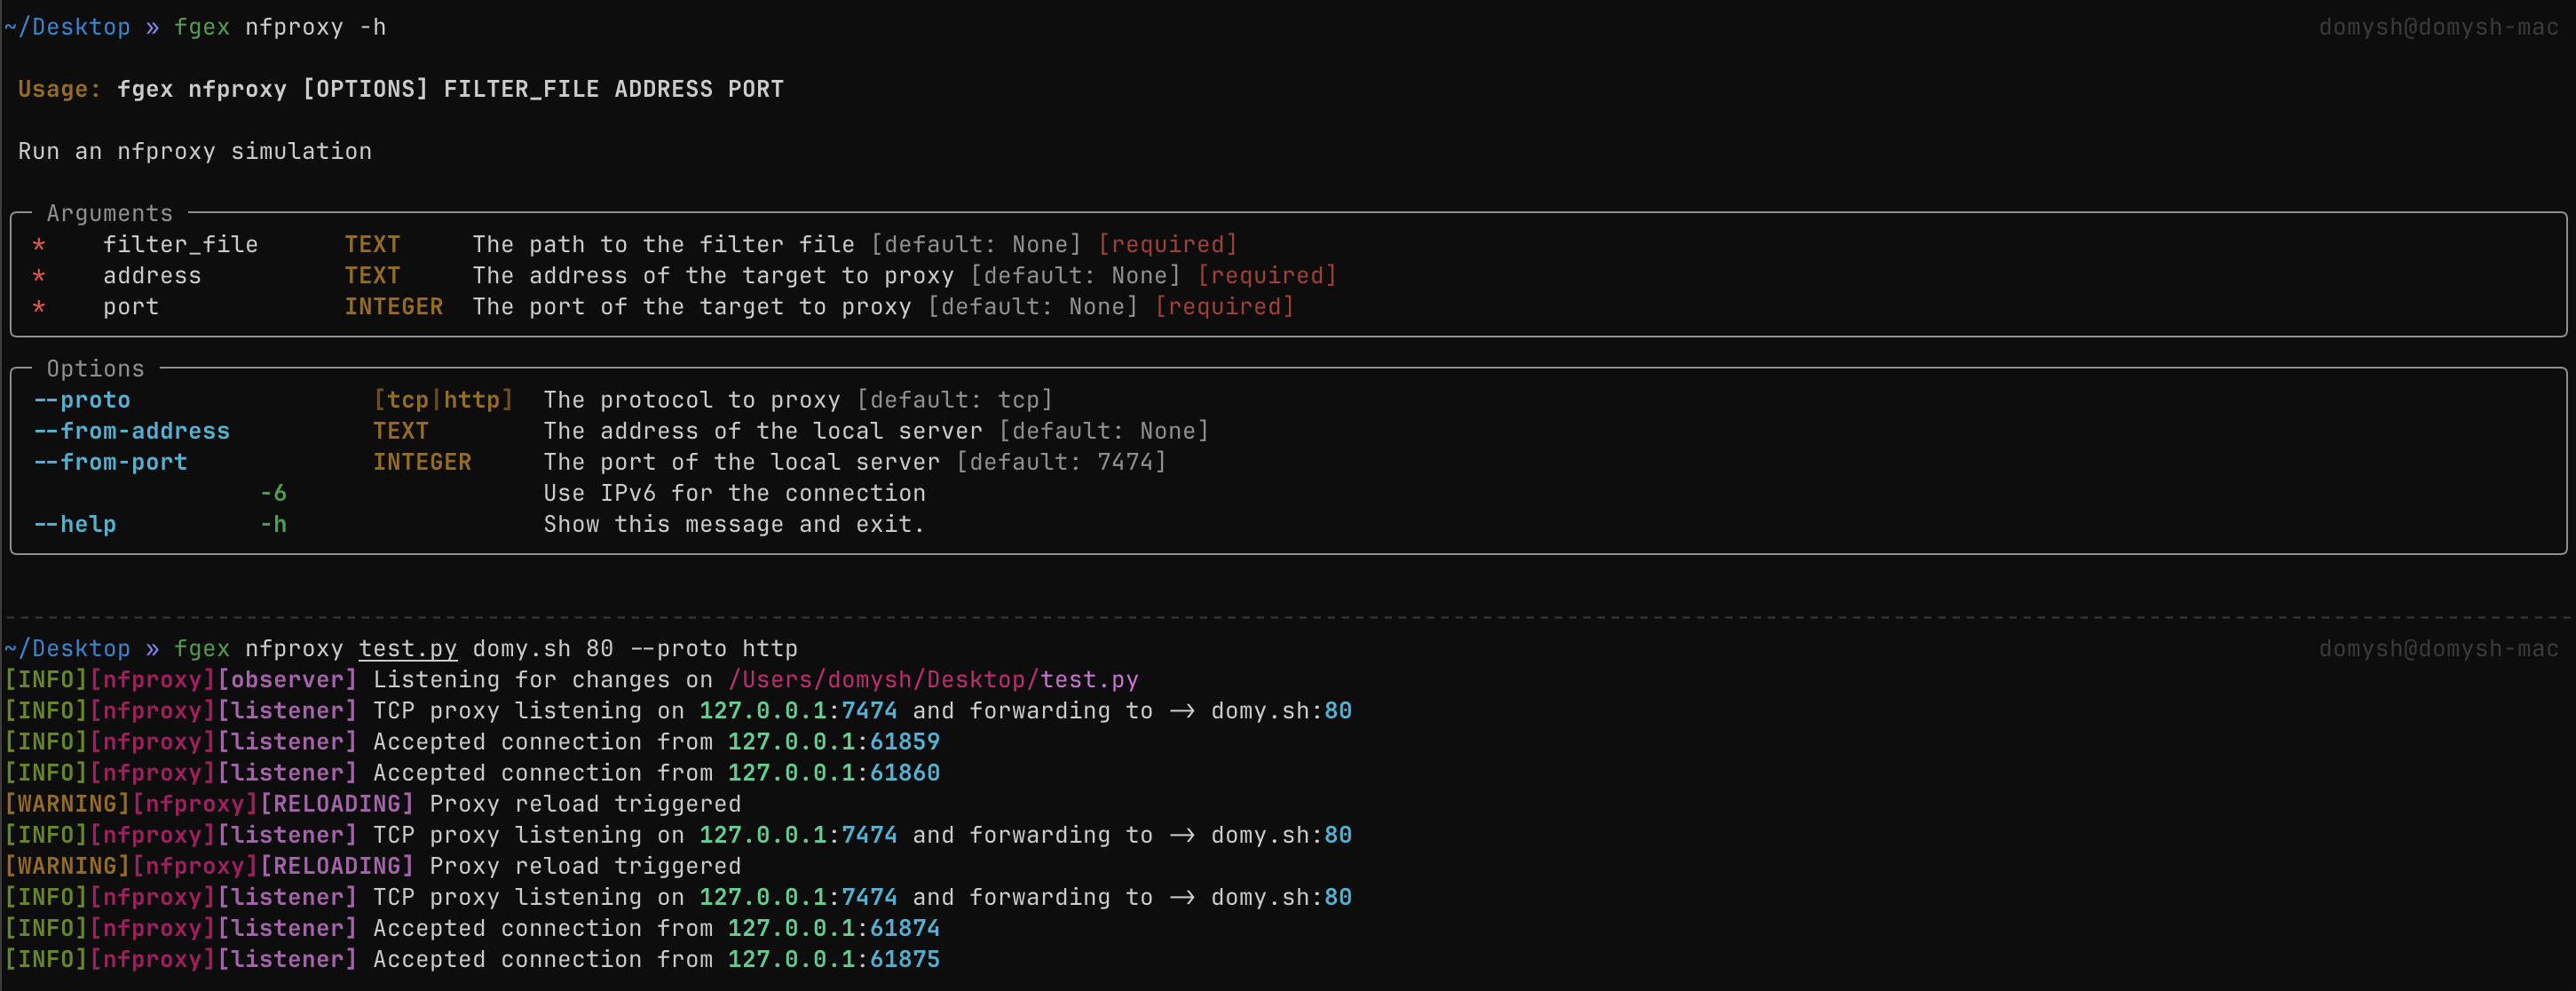
\includegraphics[width=0.98\textwidth]{images/chapter3/nfproxy_sim.png}
    \caption{Simulazione di \texttt{\gls{nfproxy}} tramite il comando fgex.}\label{fig:nfproxy_sim}
\end{figure}
